\documentclass[a4paper,12pt]{article}
\usepackage{vntex}
% vntex redefines \contentsname (and other captions) to Vietnamese by
% default; this is the English report, so switch it back.
\renewcommand{\contentsname}{Contents}
\usepackage{mathptmx}[ptm]
\usepackage{a4wide,amssymb,epsfig,latexsym,array,hhline,fancyhdr}
\usepackage[normalem]{ulem}

\usepackage[makeroom]{cancel}
\usepackage{amsmath}
\usepackage{amsthm}
\usepackage{multicol,longtable,amscd}
\usepackage{diagbox}
\usepackage{booktabs}
\usepackage{alltt}
\usepackage[framemethod=tikz]{mdframed}
\usepackage{caption,subcaption}

\usepackage{lastpage}
\usepackage{enumerate}
\usepackage{color}
\usepackage{graphicx}
\let\oldincludegraphics\includegraphics
\renewcommand{\includegraphics}[2][]{%
  \oldincludegraphics[width=\textwidth,keepaspectratio,#1]{#2}%
}
\providecommand{\pandocbounded}[1]{#1}
\usepackage{pdfpages}
\usepackage{float}
\usepackage{array}
\usepackage{tabularx, caption}
\usepackage{multirow}
\usepackage{multicol}
\usepackage{rotating}
\usepackage{geometry}
\usepackage{setspace}
\usepackage{epsfig}
\usepackage{tikz}
\usepackage{url}

\renewcommand{\arraystretch}{1.3}

\usetikzlibrary{arrows,snakes,backgrounds,calc}
\usepackage[unicode]{hyperref}
\hypersetup{urlcolor=blue,linkcolor=black,citecolor=black,colorlinks=true}
\usepackage{listings}

\IfFileExists{grffile.sty}{\usepackage{grffile}}{}

\graphicspath{{../static/images/}{Images/}}

\def\thesislayout{
	\geometry{
		a4paper,
		total={160mm,240mm},
		left=30mm,
		top=30mm,
	}
}
\thesislayout

\lstset{
basicstyle=\footnotesize\ttfamily,
breaklines=true,
breakatwhitespace=false,
frame=single,
numbers=left,
numberstyle=\tiny,
stepnumber=1,
numbersep=5pt,
tabsize=2,
showspaces=false,
showstringspaces=false,
backgroundcolor=\color{white},
captionpos=b,
}

\setlength{\headheight}{40pt}
\pagestyle{fancy}
\fancyhead{}
\fancyhead[L]{
 \begin{tabular}{rl}
    \begin{picture}(25,15)(0,0)
    \put(0,-8){
\includegraphics[width=10mm, height=10mm]{Images/hcmut.png}}
   \end{picture}&
	\begin{tabular}{l}
		\textbf{  Ho Chi Minh City University of Technology}\\
		\textbf{  Faculty of Computer Science \& Engineering}
	\end{tabular}
 \end{tabular}
}
\fancyhead[R]{
	\begin{tabular}{l}
		\tiny \bf \\
		\tiny \bf
	\end{tabular}}
\fancyfoot{}
\fancyfoot[L]{\scriptsize Off-Campus Internship Report}
\fancyfoot[R]{\scriptsize Page {\thepage}/\pageref{LastPage}}
\renewcommand{\headrulewidth}{0.3pt}
\renewcommand{\footrulewidth}{0.3pt}

\setcounter{secnumdepth}{4}
\setcounter{tocdepth}{3}
\makeatletter
\newcounter{subsubsubsection}[subsubsection]
\renewcommand\thesubsubsubsection{\thesubsubsection .\@alph\c@subsubsubsection}
\newcommand\subsubsubsection{\@startsection{subsubsubsection}{4}{\z@}%
                                     {-3.25ex\@plus -1ex \@minus -.2ex}%
                                     {1.5ex \@plus .2ex}%
                                     {\normalfont\normalsize\bfseries}}
\newcommand*\l@subsubsubsection{\@dottedtocline{3}{10.0em}{4.1em}}
\newcommand*{\subsubsubsectionmark}[1]{}
\makeatother

\everymath{\color{black}}
\sloppy
\captionsetup[figure]{labelfont={small,bf},textfont={small,it},belowskip=-1pt,aboveskip=-9pt}
\captionsetup[table]{labelfont={small,bf},textfont={small,it},belowskip=-1pt,aboveskip=7pt}
\setlength{\floatsep}{5pt plus 2pt minus 2pt}
\setlength{\textfloatsep}{5pt plus 2pt minus 2pt}
\setlength{\intextsep}{10pt plus 2pt minus 2pt}

\thesislayout

% Cover-page text sizes, held to the official template's required 15pt/18pt
% exactly. The titlepage used to overflow onto a second page; fixed via
% \coverlistspacing (tighter itemize spacing) and \enlargethispage/\vfill
% below rather than by shrinking these sizes below what's required.
\newcommand{\cover}{\fontsize{15}{18}\selectfont}
\newcommand{\coverbig}{\fontsize{18}{22}\selectfont}
\newcommand{\coverlistspacing}{\setlength{\itemsep}{2pt}\setlength{\parskip}{0pt}\setlength{\parsep}{0pt}\setlength{\topsep}{0pt}}

\begin{document}

\begin{titlepage}
\begin{tikzpicture}[remember picture, overlay]
  \draw[line width = 4pt] ($(current page.north west) + (0.4in,-0.5in)$) rectangle ($(current page.south east) + (-0.4in,0.5in)$);
  \draw[line width=1.5pt]
    ($ (current page.north west) + (0.45in,-0.55in) $)
    rectangle
    ($ (current page.south east) + (-0.45in,0.55in) $);
\end{tikzpicture}

\begin{center}
\cover \textbf{VIETNAM NATIONAL UNIVERSITY HO CHI MINH CITY} \\
\vspace{0.2cm}
\cover \textbf{HO CHI MINH CITY UNIVERSITY OF TECHNOLOGY} \\
\vspace{0.2cm}
\cover \textbf{FACULTY OF COMPUTER SCIENCE AND ENGINEERING}
\end{center}

\vspace{0.3cm}

\begin{figure}[h!]
\begin{center}

\includegraphics[width=3cm]{Images/hcmut.png}
\end{center}
\end{figure}

\begin{center}
\begin{tabular}{c}
\multicolumn{1}{c}{\textbf{{\coverbig COURSE REPORT}}}\\
\\{\textbf{{\coverbig INTERNSHIP}}}\\
\\{\textbf{{\coverbig (Course ID: CO3335)}}}
\\
\\
\textbf{\cover SEMESTER 253 ACADEMIC YEAR 2025-2026} \\
\end{tabular}
\end{center}
\vspace{0.2cm}
\begin{itemize}
\renewcommand\labelitemi{--}
\coverlistspacing
    \item \cover \textbf{MAJOR: Computer Science}
    \item \cover \textbf{TRAINING PROGRAM: OISP}
\end{itemize}
\vspace{0.35cm}
\begin{itemize}
\renewcommand\labelitemi{--}
\coverlistspacing
    \item \cover \textbf{COMPANY / INTERNSHIP UNIT:}
    \\ \cover \textbf{Amazon Web Services Viet Nam Company Limited}
    \item \cover \textbf{DIRECT SUPERVISOR AT THE COMPANY:}
    \\ \cover \textbf{Lu Hoan Thien}
    \item \cover \textbf{FACULTY SUPERVISOR / GRADER:}
    \\ \cover \textbf{Nguyen Minh Tam}
    \item \cover \textbf{STUDENTS:}
    \\ \cover \textbf{FULL NAME: Nguyen Thanh Tai} \textbf{STUDENT ID: 2353062}
\end{itemize}
% Push the place/date line down to the foot of the cover. \enlargethispage
% reaches past the normal text block so the line can sit just inside the
% border; \vfill collapses harmlessly if the cover ever grows.
\enlargethispage{1.3cm}
\vfill
\begin{center}
{\cover HO CHI MINH CITY, AUGUST 2026}
\end{center}
\vspace{0.5cm}
\end{titlepage}

\newpage
\tableofcontents
\newpage

% No printed heading on this page (the scanned form starts immediately),
% but it still gets a numbered entry in the table of contents matching
% what \section would have produced.
\stepcounter{section}
\phantomsection
\addcontentsline{toc}{section}{\protect\numberline{\thesection}Internship Program}

\IfFileExists{form/formD2.pdf}{
  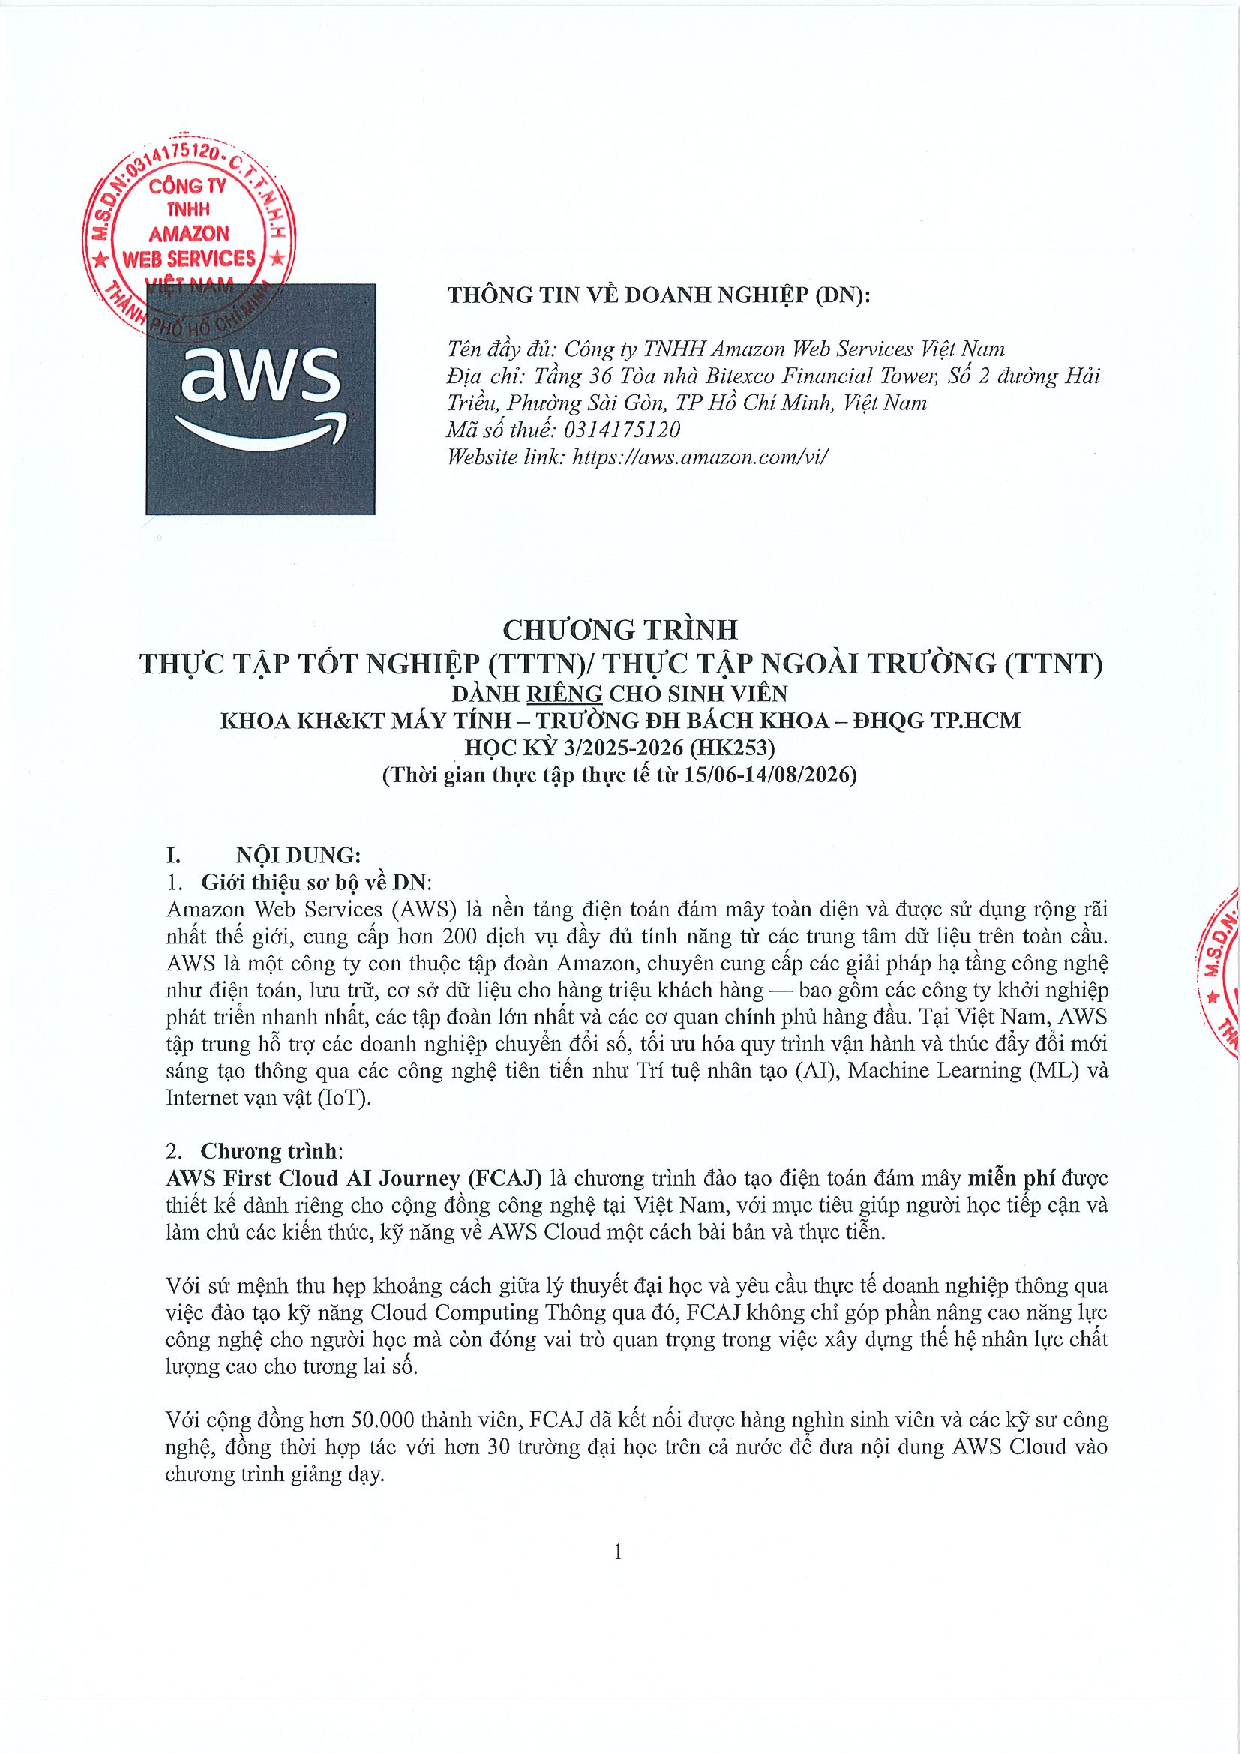
\includepdf[pages=-,pagecommand={\thispagestyle{empty}}]{form/formD2.pdf}
}{
    \pagebreak
    \begin{center}
        \textit{Attach form D2 here}
    \end{center}
    \pagebreak
}

\thispagestyle{fancy}
\setcounter{page}{\thepage}

\endinput

% No printed heading on this page (the scanned form starts immediately),
% but it still gets a numbered entry in the table of contents matching
% what \section would have produced.
\stepcounter{section}
\phantomsection
\addcontentsline{toc}{section}{\protect\numberline{\thesection}Admission Results}

\IfFileExists{form/formD3.pdf}{
  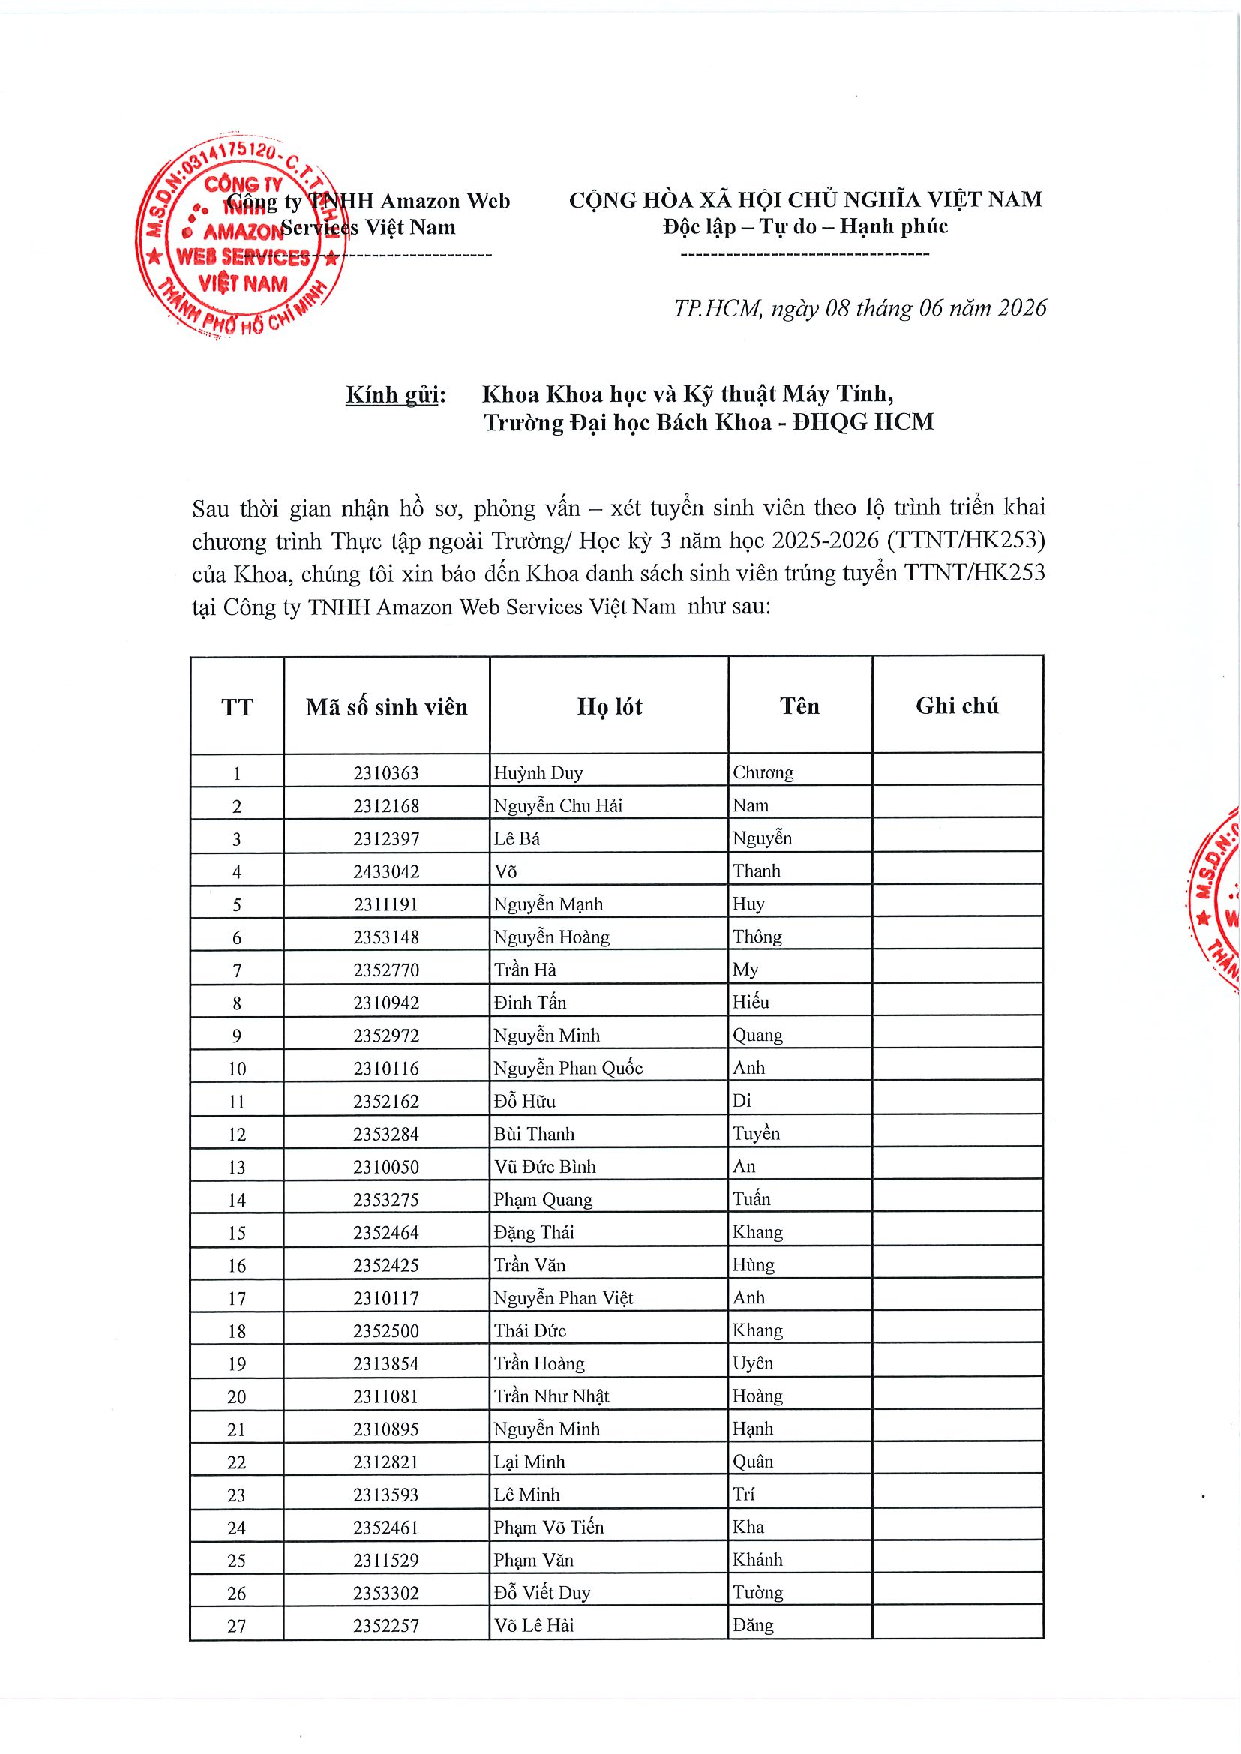
\includepdf[pages=-,pagecommand={\thispagestyle{empty}}]{form/formD3.pdf}
}{
    \pagebreak
    \begin{center}
        \textit{Attach form D3 here}
    \end{center}
    \pagebreak
}

\thispagestyle{fancy}
\setcounter{page}{\thepage}

\endinput

\input{generated/content_body_en}

\newpage
\section{Summary}

\subsection{Skills and knowledge gained}

During my internship at \textbf{Amazon Web Services Vietnam Company Limited} from \textbf{15/06/2026} to \textbf{31/07/2026}, as part of the Workforce Bootcamp - First Cloud Journey programme, I had the opportunity to move from studying cloud computing in theory to designing, building, and operating a complete system on AWS.

The project - \textbf{Caerus}, a cinema seat booking platform built by a two-person team - was chosen in the first week, not left until later: the API specification and database schema were agreed and frozen before any AWS service was studied in depth. The two weeks after that covered the core AWS fundamentals needed to build it; the remaining four weeks built the application, deployed it, removed its single points of failure, and put monitoring in place. The final architecture runs across Amazon EC2 (two instances, private subnets, behind an Application Load Balancer and a NAT gateway), Amazon RDS for PostgreSQL (Multi-AZ, private subnet), Amazon S3, Amazon CloudFront with AWS WAF, AWS Systems Manager, and Amazon CloudWatch with SNS - having tried, and deliberately removed, AWS Lambda and API Gateway for ticket generation along the way once the evidence showed a persistent server was the better fit.

Through this work I improved my skills in cloud architecture and service selection, relational database design, transactional programming and concurrency control, API design, deployment and network security configuration, observability, cost management, and technical documentation. Working in a pair also taught me the value of agreeing an interface contract before writing code, which is what allowed two people to build simultaneously rather than one waiting on the other.

In terms of work ethic, I kept to the schedule agreed at the start of the project, maintained the daily habits the team committed to - terminating practice resources the same day and tagging every resource with its owner - and raised problems with my teammate early rather than working around them alone.

\subsection{What went well}

\begin{itemize}
    \item \textbf{Learning breadth.} I began the programme with no practical AWS experience and finished it able to design a multi-service architecture and justify each service choice against an alternative rather than by default.
    \item \textbf{Working from a contract.} Agreeing the API specification and database schema before writing any code was the single decision that kept the project on schedule. It meant the frontend was never blocked waiting for the backend, and it made integration a matter of fixing small mismatches rather than reconciling two incompatible designs.
    \item \textbf{Solving the problem the project was actually about.} Seat booking under concurrency is not a user-interface problem or an infrastructure problem; it is a transaction problem. I learned to lock the contested rows explicitly, order the locks consistently to avoid deadlocks, and then prove the guarantee with a deliberate two-client race rather than assuming it held.
    \item \textbf{Revising decisions on evidence.} We moved booking cancellation to a Lambda function, then moved it back once it became clear cancellation shares its transaction logic with booking and gained nothing from being split out. Ticket generation went further: we built it as a Lambda function, deployed it, confirmed it worked correctly, and removed it anyway once the workload turned out too small and infrequent to justify a second deployable with its own IAM role and deploy step. Recording that reasoning rather than quietly reverting was the habit worth keeping, not the reversal itself.
    \item \textbf{Cost discipline.} Setting a billing alarm before provisioning anything, tagging every resource with an owner, and later raising the alarm threshold to match the architecture's real run-rate once the load balancer, the NAT gateway, and a Multi-AZ database made the original Free Tier estimate inaccurate, meant cost stayed a known, monitored number throughout rather than a surprise reconstructed after the fact.
\end{itemize}

\subsection{What I would do differently}

\begin{itemize}
    \item \textbf{Proactiveness beyond the plan.} I executed the agreed schedule reliably, but I tended to work through the task list rather than looking ahead and proposing improvements before they became necessary. Several issues we hit during deployment were foreseeable, and I should have raised them at design time instead of discovering them under time pressure.
    \item \textbf{Communication and presentation.} I am comfortable explaining technical decisions in writing, but less confident presenting them verbally to an audience that has not read the documents. This is the skill I would most like to develop next.
    \item \textbf{Verifying the edge layer for every request shape, not just the happy path.} When CloudFront and its bundled WAF went in front of the API, testing covered page loads and ordinary JSON calls, but not a large multipart file upload going through the same path. A poster upload silently failed in the deployed environment - blocked by a default WAF body-size rule, then disguised as a fake success by the distribution's own SPA-fallback error response - and it took real debugging afterward to find. I now treat "this layer works" as meaning it works for every request shape the application actually sends, not just the first one I happened to try.
    \item \textbf{Depth beyond the working path.} The system works and is verified against its core guarantee, but the engineering around it is thinner than I would like: deployment is manual rather than automated (no CI/CD pipeline), and infrastructure was created through the console rather than defined as code, which makes the environment harder to reproduce exactly than it should be.
    \item \textbf{Estimating time.} My original estimates for deployment and cross-origin configuration were optimistic. The buffer days built into the plan absorbed the overrun, but the estimates themselves need to improve.
\end{itemize}

\subsection{Self-assessment}

\begingroup
\small
\setlength{\tabcolsep}{4pt}
\renewcommand{\arraystretch}{1.2}
\begin{longtable}{@{}p{0.03\linewidth}p{0.20\linewidth}p{0.47\linewidth}ccc@{}}
\toprule
\textbf{No.} & \textbf{Criteria} & \textbf{Description} & \textbf{Good} & \textbf{Fair} & \textbf{Avg.} \\
\midrule
\endhead
\bottomrule
\endfoot
1 & Professional knowledge \& skills & Understanding of the field, applying knowledge in practice, proficiency with tools, work quality & $\checkmark$ & $\square$ & $\square$ \\
2 & Ability to learn & Ability to absorb new knowledge and learn quickly & $\checkmark$ & $\square$ & $\square$ \\
3 & Proactiveness & Taking initiative, seeking out tasks without waiting for instructions & $\square$ & $\checkmark$ & $\square$ \\
4 & Sense of responsibility & Completing tasks on time and ensuring quality & $\checkmark$ & $\square$ & $\square$ \\
5 & Discipline & Adhering to schedules, rules, and work processes & $\checkmark$ & $\square$ & $\square$ \\
6 & Progressive mindset & Willingness to receive feedback and improve oneself & $\checkmark$ & $\square$ & $\square$ \\
7 & Communication & Presenting ideas and reporting work clearly & $\square$ & $\checkmark$ & $\square$ \\
8 & Teamwork & Working effectively with colleagues and participating in teams & $\checkmark$ & $\square$ & $\square$ \\
9 & Professional conduct & Respecting colleagues, partners, and the work environment & $\checkmark$ & $\square$ & $\square$ \\
10 & Problem-solving skills & Identifying problems, proposing solutions, and showing creativity & $\checkmark$ & $\square$ & $\square$ \\
11 & Contribution to project/team & Work effectiveness, innovative ideas, recognition from the team & $\checkmark$ & $\square$ & $\square$ \\
12 & Overall & General evaluation of the entire internship period & $\checkmark$ & $\square$ & $\square$ \\
\end{longtable}
\endgroup

% Signed signature page. Falls back to a hand-drawn placeholder (matching
% the D2/D3 form pattern) if the scanned/rendered PDF isn't present.
\IfFileExists{form/TongKet.pdf}{
  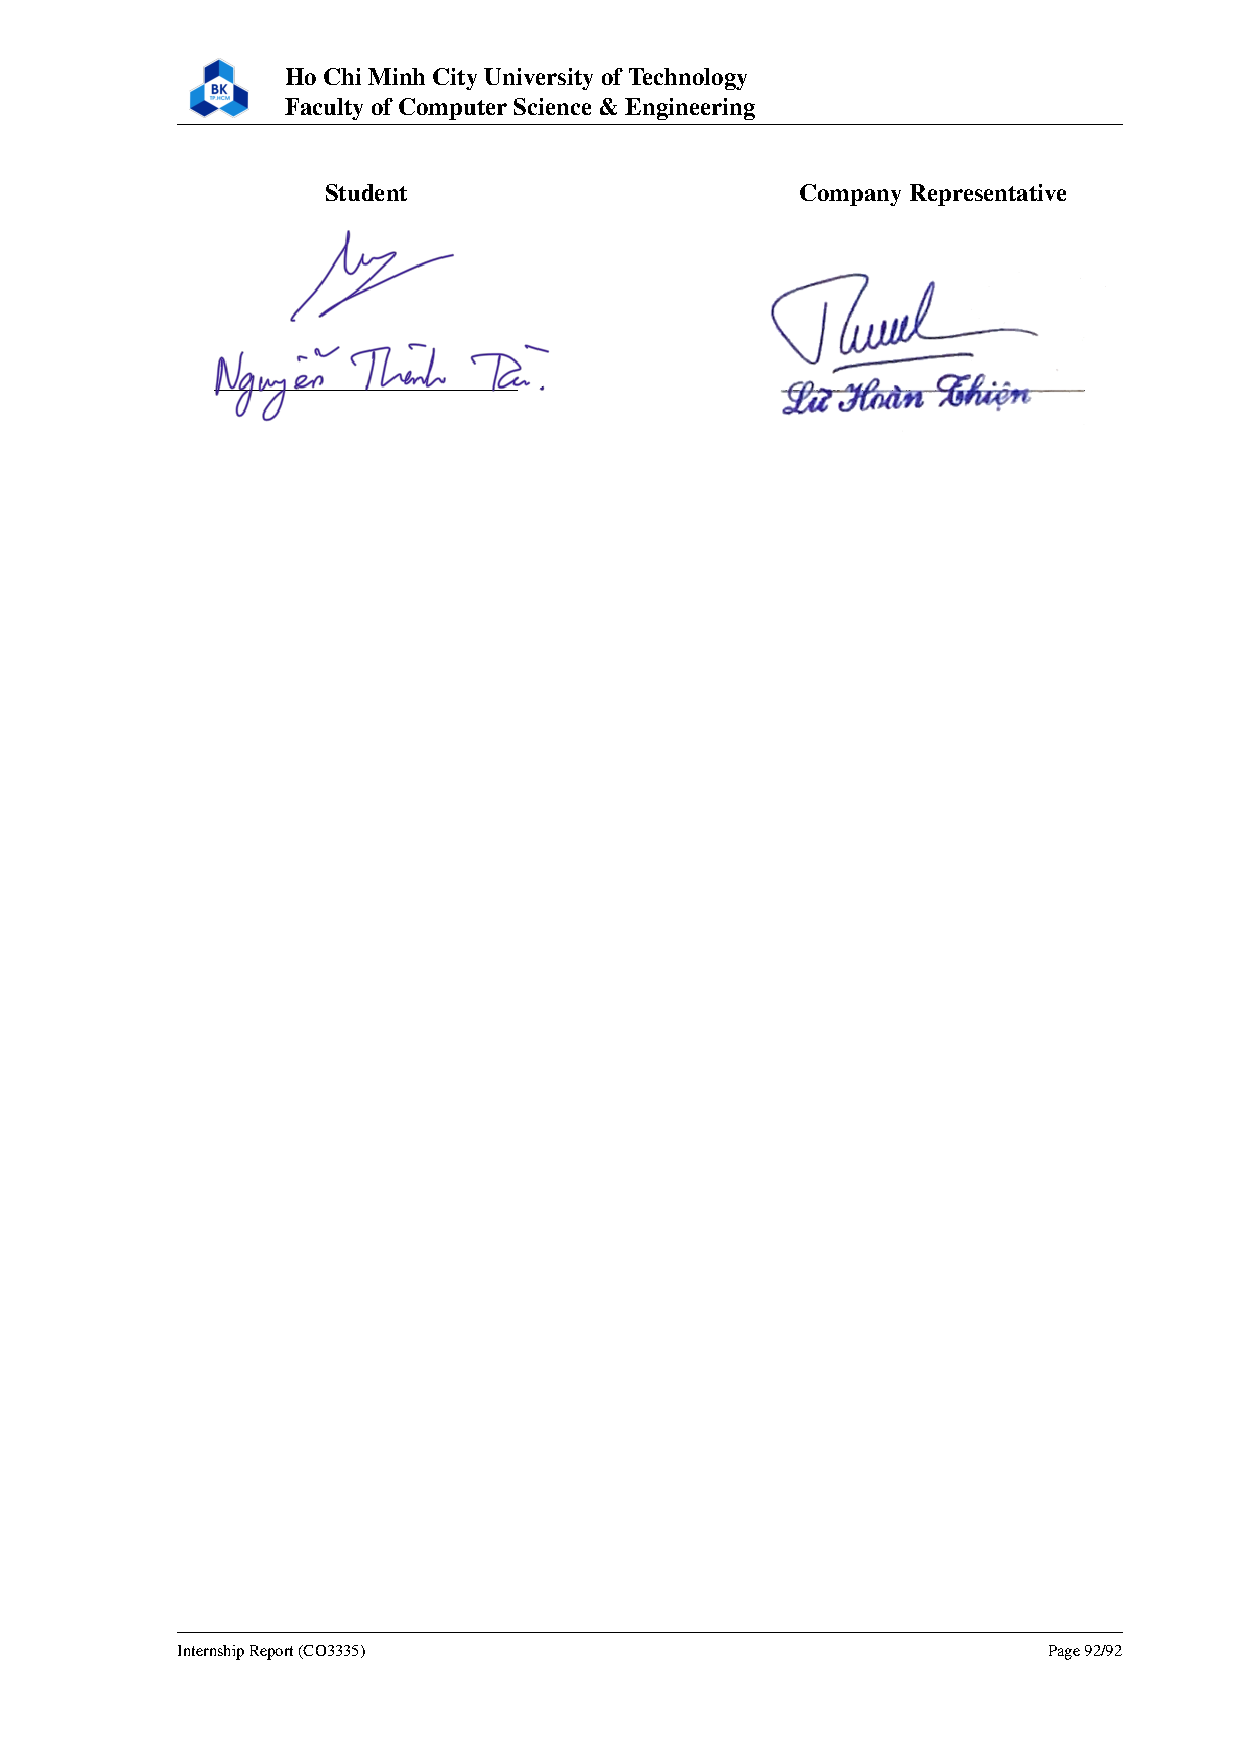
\includepdf[pages=-,pagecommand={\thispagestyle{empty}}]{form/TongKet.pdf}
}{
\newpage
\vspace{1cm}

\begin{center}
\begin{minipage}[t]{0.4\textwidth}
    \centering
    \textbf{Student}\\[0.2cm]
    % (Signature and full name)

    \vspace{2.5cm}

    \rule{0.8\linewidth}{0.4pt}
\end{minipage}
\hfill
\begin{minipage}[t]{0.4\textwidth}
    \centering
    \textbf{Company Representative}\\[0.2cm]
    % (Signature and full name)

    \vspace{2.5cm}

    \rule{0.8\linewidth}{0.4pt}
\end{minipage}
\end{center}
}
\end{document}
